\documentclass[11pt,border=6pt]{standalone}
\usepackage{fontspec}
\usepackage{tikz}
\usetikzlibrary{positioning,arrows.meta,calc,fit}
\begin{document}
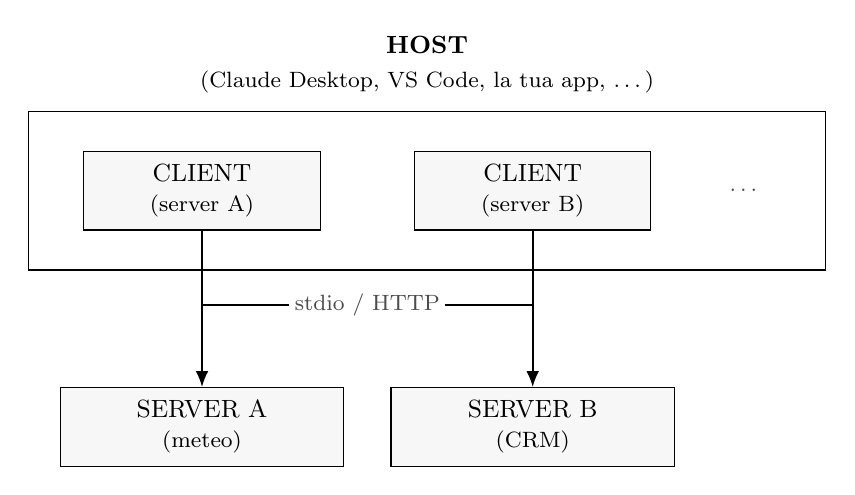
\begin{tikzpicture}[font=\small,
  cli/.style={draw, minimum width=3.0cm, minimum height=10mm, align=center, fill=black!3},
  srv/.style={draw, minimum width=3.6cm, minimum height=10mm, align=center, fill=black!3},
  arr/.style={-{Latex[length=2mm,width=1.6mm]}, semithick},
  note/.style={font=\footnotesize, text=black!70}]

  \node[cli] (cliA) at (0,0) {CLIENT\\\footnotesize (server A)};
  \node[cli] (cliB) at (4.2,0) {CLIENT\\\footnotesize (server B)};
  \node[note] (dots) at (6.9,0) {\dots};

  \node[draw, fit=(cliA)(cliB)(dots), inner xsep=7mm, inner ysep=5mm,
        label={[font=\small, align=center, yshift=3pt]above:{\textbf{HOST}\\[1pt]
          \footnotesize (Claude Desktop, VS Code, la tua app, \dots)}}] (host) {};

  \node[srv] (srvA) at (0,-3.0) {SERVER A\\\footnotesize (meteo)};
  \node[srv] (srvB) at (4.2,-3.0) {SERVER B\\\footnotesize (CRM)};

  \draw[semithick] (cliA.south) -- (0,-1.45) -- (4.2,-1.45) -- (cliB.south);
  \node[note, fill=white, inner sep=2pt] at (2.1,-1.45) {stdio / HTTP};
  \draw[arr] (0,-1.45) -- (srvA.north);
  \draw[arr] (4.2,-1.45) -- (srvB.north);
\end{tikzpicture}
\end{document}

